\begin{figure}[t]
\centering
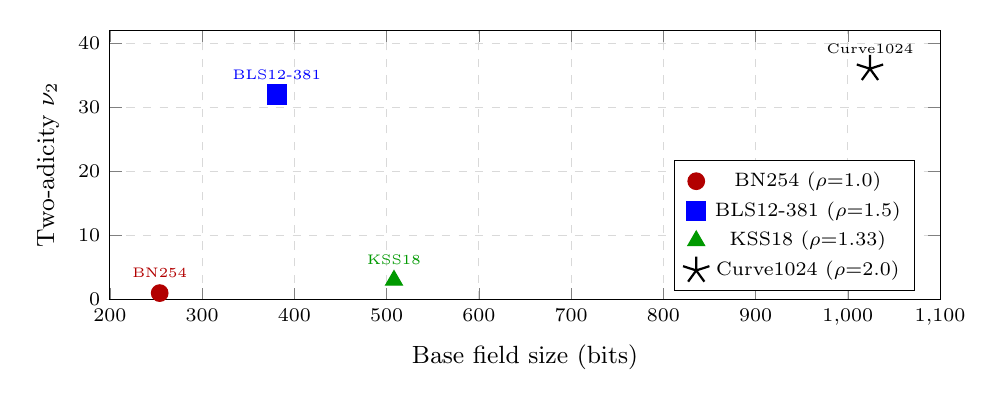
\begin{tikzpicture}
\begin{axis}[
    width=\columnwidth,
    height=5cm,
    xlabel={Base field size (bits)},
    ylabel={Two-adicity $\nu_2$},
    xmin=200, xmax=1100,
    ymin=0, ymax=42,
    grid=major,
    grid style={dashed, gray!30},
    every axis label/.style={font=\small},
    tick label style={font=\scriptsize},
    legend pos=south east,
    legend style={font=\scriptsize},
]
% BN254
\addplot[only marks, mark=*, mark size=3pt, color=red!70!black] coordinates {(254, 1)};
\addlegendentry{BN254 ($\rho{=}1.0$)}

% BLS12-381
\addplot[only marks, mark=square*, mark size=3.5pt, color=blue] coordinates {(381, 32)};
\addlegendentry{BLS12-381 ($\rho{=}1.5$)}

% KSS18
\addplot[only marks, mark=triangle*, mark size=3.5pt, color=green!60!black] coordinates {(508, 3)};
\addlegendentry{KSS18 ($\rho{=}1.33$)}

% Curve1024
\addplot[only marks, mark=star, mark size=5pt, color=black, line width=0.8pt] coordinates {(1024, 36)};
\addlegendentry{Curve1024 ($\rho{=}2.0$)}

% Labels above points
\node[font=\tiny, above=2pt, red!70!black] at (axis cs:254,1) {BN254};
\node[font=\tiny, above=2pt, blue] at (axis cs:381,32) {BLS12-381};
\node[font=\tiny, above=2pt, green!60!black] at (axis cs:508,3) {KSS18};
\node[font=\tiny, above=2pt] at (axis cs:1024,36) {Curve1024};
\end{axis}
\end{tikzpicture}
\caption{Pairing-friendly curve comparison: field size vs.\ two-adicity. Curve1024 achieves the highest two-adicity (36) and ECDLP security (256-bit) at the cost of a larger $\rho$-value.}
\label{fig:comparison}
\end{figure}
